\documentclass[12pt]{article}

\usepackage{amssymb,amsmath,amsfonts,eurosym,geometry,ulem,graphicx,caption}
\usepackage{color,setspace,sectsty,comment,footmisc,caption,pdflscape,subfigure}
\usepackage{array,hyperref,authblk}
\usepackage{makecell}
\usepackage{apacite}
\usepackage{algorithm,algorithmic}
\usepackage [english]{babel}
\usepackage [autostyle, english = american]{csquotes}
\MakeOuterQuote{"}

\graphicspath{ {../charts/} }

\renewcommand\theadalign{cc}
\renewcommand\theadfont{\bfseries}
\renewcommand\theadgape{\Gape[4pt]}
\renewcommand\cellgape{\Gape[4pt]}

%\normalem

\onehalfspacing
\newtheorem{theorem}{Theorem}
\newtheorem{corollary}[theorem]{Corollary}
\newtheorem{proposition}{Proposition}
\newenvironment{proof}[1][Proof]{\noindent\textbf{#1.} }{\ \rule{0.5em}{0.5em}}

\newtheorem{hyp}{Hypothesis}
\newtheorem{subhyp}{Hypothesis}[hyp]
\renewcommand{\thesubhyp}{\thehyp\alph{subhyp}}

\newcommand{\red}[1]{{\color{red} #1}}
\newcommand{\blue}[1]{{\color{blue} #1}}

\newcolumntype{L}[1]{>{\raggedright\let\newline\\arraybackslash\hspace{0pt}}m{#1}}
\newcolumntype{C}[1]{>{\centering\let\newline\\arraybackslash\hspace{0pt}}m{#1}}
\newcolumntype{R}[1]{>{\raggedleft\let\newline\\arraybackslash\hspace{0pt}}m{#1}}

\geometry{left=1.0in,right=1.0in,top=1.0in,bottom=1.0in}

\begin{document}

\begin{titlepage}
\title{Optimal transfer targeting and universal basic income with noisy data}
\author{Max Ghenis\thanks{Affiliations: Massachusetts Institute of Technology 
and UBI Center (max@ubicenter.org).
\protect \\
\protect \\Thanks to Ben Olken for helpful comments.
}}

\date{April 8, 2020}
\maketitle
\begin{abstract}
\noindent \citeA{hannaolken} found that targeting transfers to households 
predicted to be poor achieves greater social welfare than universal targeting, 
in contexts of Indonesia and Peru with noisy consumption data and fixed program 
budgets. I extend this by varying three components: program budget, amount of 
noise, and the share of the budget dedicated to a universal transfer (universal 
basic income, or UBI). Using data from the US Current Population Survey, my 
simulations show that reserving a portion of the budget for UBI improves social 
welfare, especially with larger budgets and with noisier data.

\bigskip
\end{abstract}
\setcounter{page}{0}
\thispagestyle{empty}
\end{titlepage}
\pagebreak \newpage




\doublespacing


\section{Introduction} \label{sec:introduction}

How narrowly or broadly to target transfer programs is a central question
in public finance, especially in developing countries with highly constrained
government budgets and difficulty implementing phase-outs more common
in developed country safety net programs.
On one hand, narrow targeting concentrates resources on those in greatest need;
on the other, excluding those just above the threshold might miss opportunities
to reduce poverty.
This challenge is further complicated by imprecise household surveys used to
target these programs, which must be administered widely.

To weigh these trade-offs, \citeA{hannaolken} (\textit{H-O})
paired household surveys from the Indonesian and Peruvian governments with more 
detailed consumption surveys showing a ground truth signal of consumption.
This enabled them to predict actual consumption from simpler surveys that can
be used for program targeting,
and to estimate the precision of these predictions.

\begin{center}
	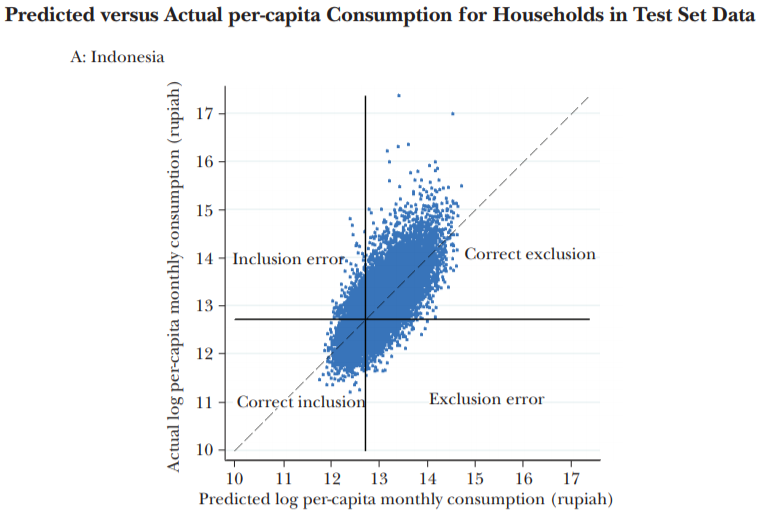
\includegraphics[width=15cm]{../img/hanna_olken_2018_pred_actual_cons}
	% Otherwise the wrapped line isn't centered.
	\captionsetup{justification=centering}
	\captionof{figure}{Predicted versus Actual per-capita Consumption for 
	Households in Test Set Data, Indonesia \protect\cite{hannaolken}}
	\label{fig:ho_pred_actual_cons}
\end{center}

Their regressions (on log per capita
consumption\footnote{Per the appendix in \citeA{hannaolken}.})
were moderately accurate, with $R^2$ values between 0.53 and 0.66.
Given this imperfect targeting data, they estimate the effect on social
welfare of targeting at different thresholds in comparison to universal basic
incomes.

They apply the constant relative risk-aversion CRRA total social welfare 
utility function:

\begin{equation}
U = \frac{\sum{(y_i + b_i)^{1-\rho}}}{1-\rho}
\end{equation}

Where $\rho$ indicates the social weight of lower-consumption households.
Using $\rho = 3$, they find the total social welfare as a function 
of the targeted share of the population. The below chart uses inclusion error 
on the x axis for comparison between Indonesia and Peru; this moves with the 
share of the population receiving the transfer.

\begin{center}
	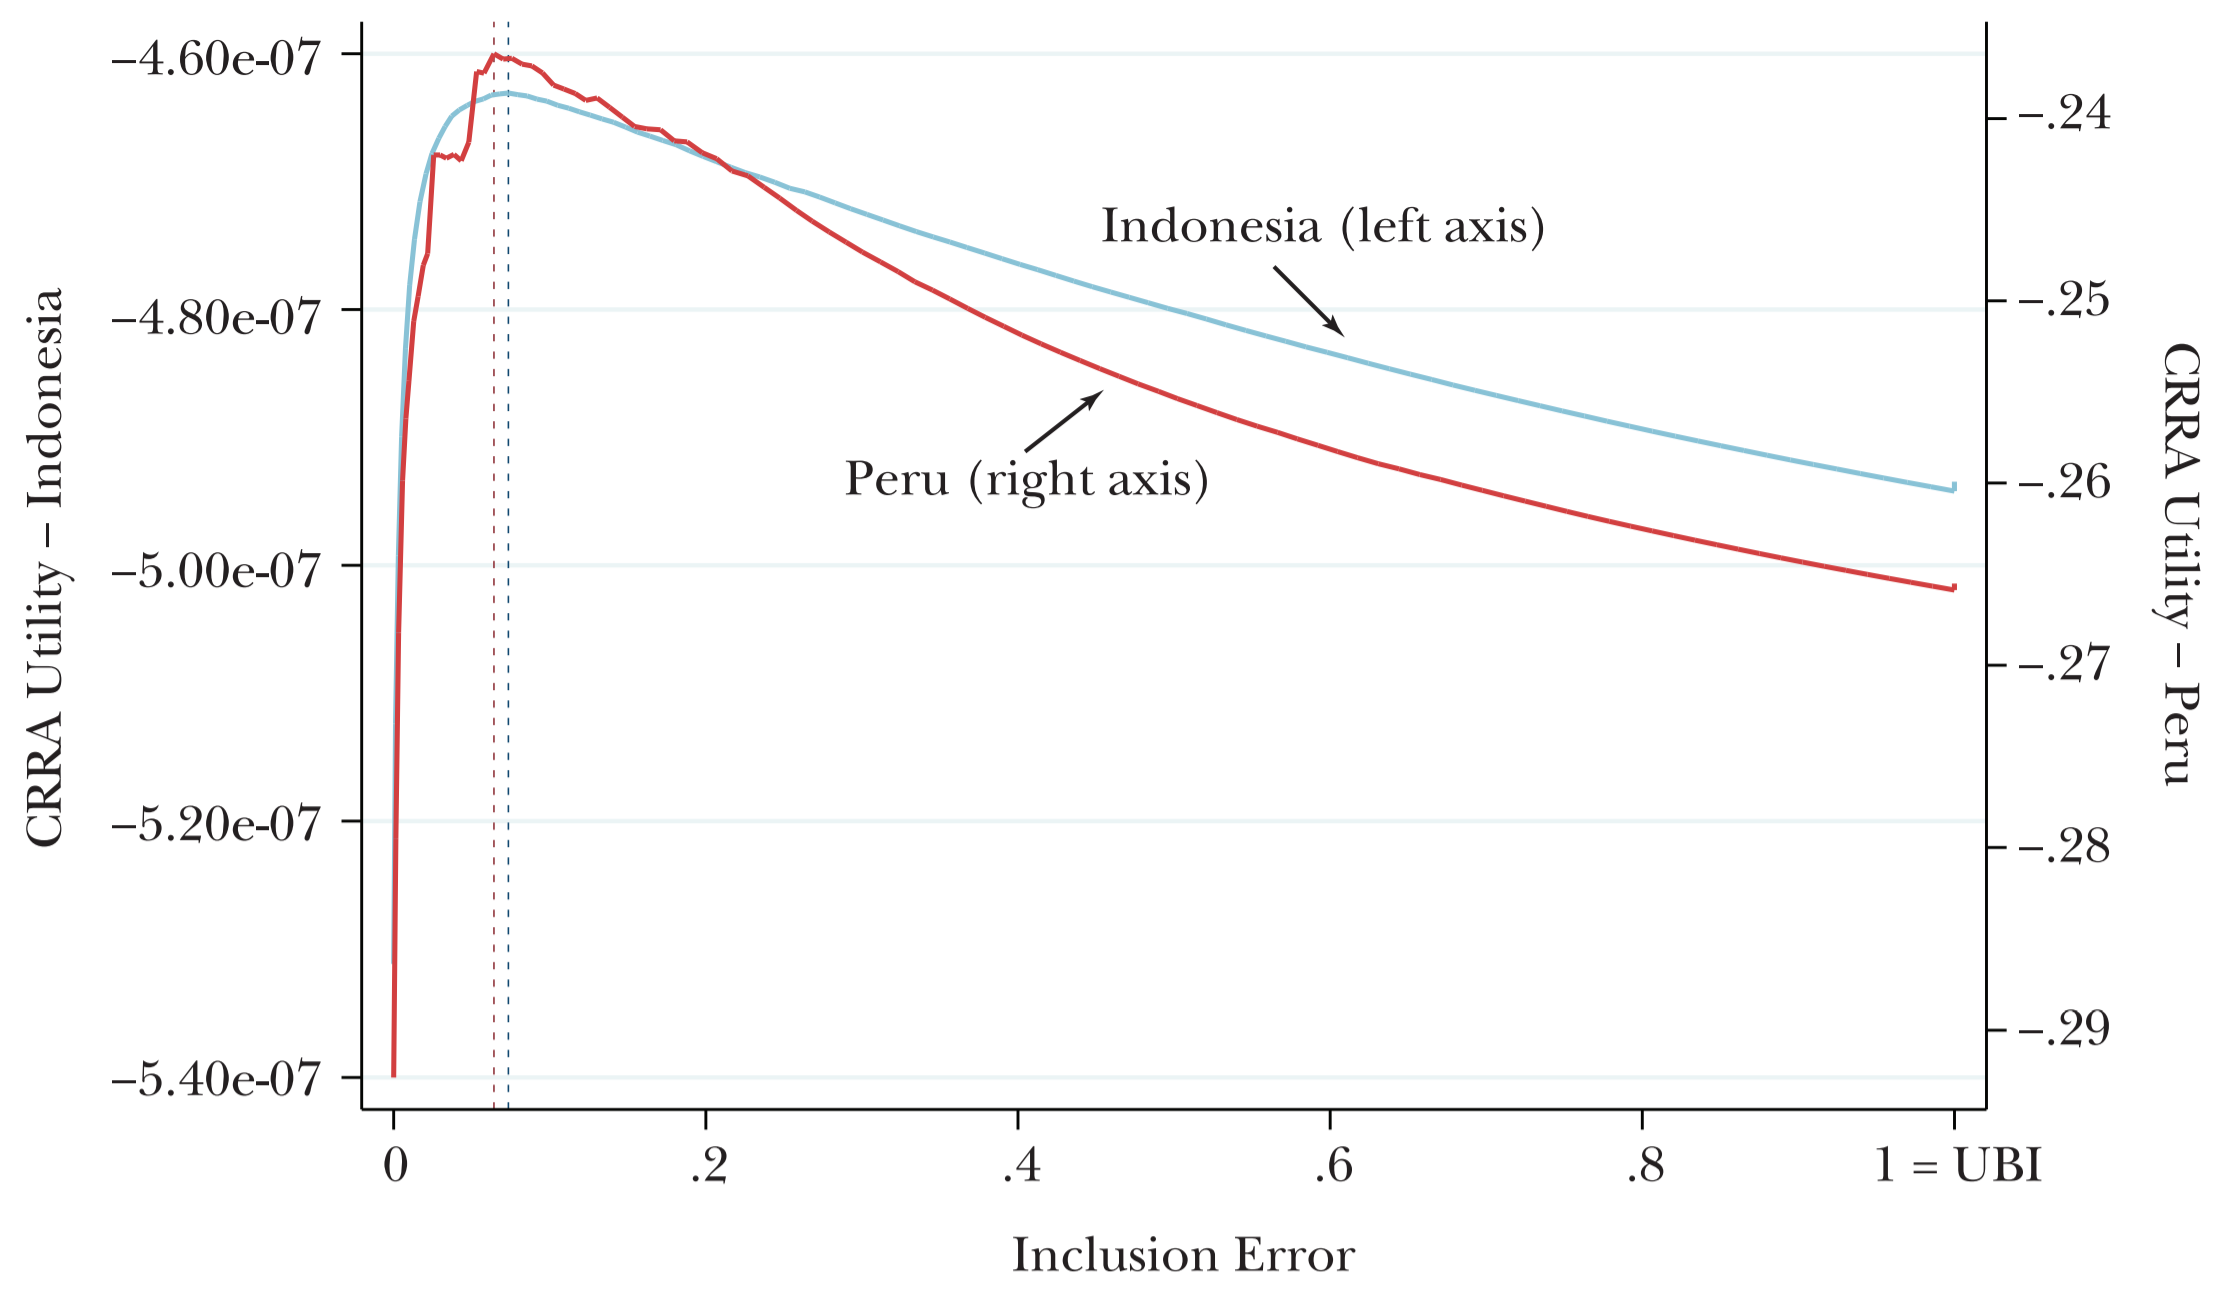
\includegraphics[width=15cm]{../img/hanna_olken_2018_social_welfare_vs_inclusion_error}
	\captionof{figure}{Social Welfare versus Inclusion Error 
	\protect\cite{hannaolken}}
	\label{fig:ho_sw_inclusion_error}
\end{center}

They find: "In Indonesia, the socially optimal program calculated in this way 
targets about 19 percent of the population, with inclusion error of 7.4 percent 
and exclusion error of 58.2 percent; for Peru, the socially optimal program 
targets approximately 18 percent of the population, with inclusion error of 6.4 
percent and exclusion error of 52.4 percent."

These are based on "a fixed transfer budget of approximately \$1.83 billion per 
year in Indonesia and \$274 million per year in Peru (modeled after the sizes 
of BLT and Juntos, respectively)" and survey years 2010-2011. As of 2011, 
Indonesia's GDP was \$893 billion and Peru's GDP was \$172 billion \cite{wb}.
These budgets were therefore 0.20 percent of GDP in Indonesia and 0.16 percent 
of GDP in Peru.
In the context of the United States in 2018, where GDP was \$20.5 
trillion,
these programs would be equivalent to \$32 billion and \$40 billion.


\section{Data} \label{sec:data}

I use data from the 2019 US Current Population Survey March
Supplement \cite{asec}, 
considering total 2018 resources from the Supplemental Poverty Measure
(\textit{SPM}) \cite{spm}.
I divide data by "SPM unit," a type of household unit created by the Census 
Bureau to estimate groups that share resources,
and divide each SPM unit's income after taxes and transfers (\textit{income})
by the number of people in the SPM unit.
This approach mirrors H-O's usage of household-level per-capita consumption 
data.

I set nonpositive per-capita income to \$1.

I simulate noise by adding random normal values to $\ln{income}$, and 
exponentiating the result.
The mean of the noise is adjusted to produce a 
similar $R^2$ result (on $\ln{income}$) to H-O (0.595, achieved with a mean of 
1.37).
This is the "low" level of noise; "high" noise has double the noise mean.


\section{Methodology} \label{sec:methodology}

For a given program budget, targeting threshold (as percent of households), 
share of budget directed to UBI, and noise level, each household is assigned a 
transfer amount. First, each household gets an equal share of the UBI 
component. Households with a predicted income percent rank (i.e., based on 
potentially noisy data) below the targeting threshold also get an equal share 
of the remaining budget.

Given original income and the transfer amount, I calculate the CRRA with 
$\rho=3$.

This is performed for 6 * 3 * 101 * 101 = 183,618 simulations, crossing the 
following variables:

\begin{itemize}
	
	\item Budget levels as a share of 2018 US GDP of 0.01\%, 0.1\%, 0.2\% 
	(closest to 
	Indonesia's BLT budget), 0.5\%, 1\%, and 5\%. Respectively, this equates to 
	\$2.05, \$20.5, \$41, \$102.5, \$205, and \$1,025 billion USD.
	
	\item Noise levels of none, low (similar to H-O prediction model), and high 
	(double the noise of H-O).
	
	\item Targeting thresholds between 0\% and 100\%, in 1\% increments.
	
	\item UBI shares between 0\% and 100\%, in 1\% increments.
	
\end{itemize}


\section{Results} \label{sec:results}

The most comparable simulation to H-O's Indonesia and Peru cases is a program 
budgeted to 0.2 percent of GDP with "low" noise (matching their $R^2$). In this 
case, the optimal policy targets 11 percent of the population. 

\begin{center}
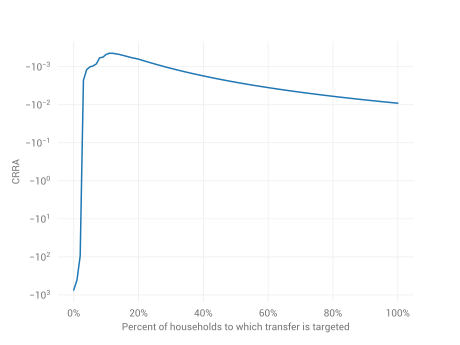
\includegraphics{single_plot_0_2_0_Low_noise}  % [width=15cm] 
\captionof{figure}{CRRA by share given transfer, 0.2\% of GDP, low 
noise\protect\footnotemark}
\label{fig:single_plot_0_2_0_Low_noise}
\end{center}

\footnotetext{I plot CRRA on a log y scale, where H-O plot it on a linear y 
scale.}

Using this as a baseline, we can see how the three types of variation affect 
the optimal targeting.

\subsection{Varying by budget} \label{varying_by_budget}

Larger program budgets enable greater social welfare, and are best distributed 
to larger portions of the population.

\begin{center}
	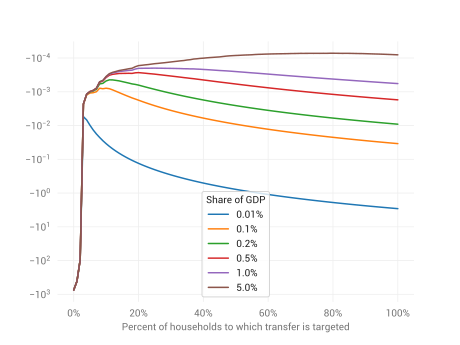
\includegraphics{by_budget_0_Low_noise}  % [width=15cm] 
	\captionof{figure}{CRRA by share given transfer and program size, low noise}
	\label{fig:by_budget_0_Low_noise}
\end{center}

Optimal social welfare rises roughly linearly in log-log space with respect to 
the program budget for each of the noise categories. For large program budgets, 
the scenarios converge by noise level as all target larger portions of the 
population.

\begin{center}
	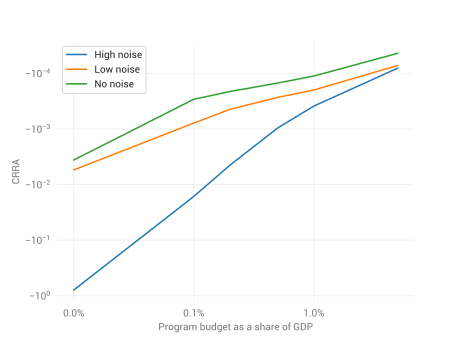
\includegraphics{max_crra_by_size_noise}  % [width=15cm] 
	\captionof{figure}{Maximum social welfare by program size and noise}
	\label{fig:max_crra_by_size_noise}
\end{center}

Larger programs achieve greater social welfare when they are less targeted, 
especially when moving from 1 to 5 percent of GDP. A program budgeted for 5 
percent of GDP should be universal if the signal is noisy, and even if the 
signal is perfect, it should be distributed to nearly half the population.

\begin{center}
	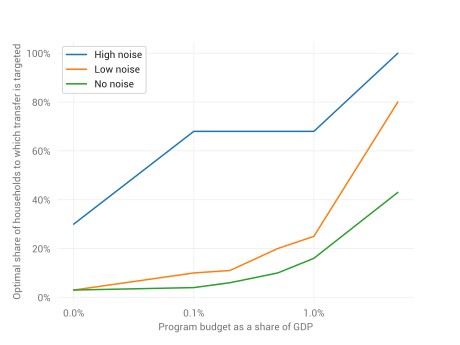
\includegraphics{optimal_targeting_by_size_noise}  % [width=15cm] 
	\captionof{figure}{Optimal targeting by program size and noise}
	\label{fig:optimal_targeting_by_size_noise}
\end{center}

\subsection{Varying by noise level} \label{varying_by_noise}

The more noisy the signal, the better it is to include a larger population 
share. With no noise, welfare is optimized when targeting 6 percent of the 
population; with low noise (H-O level), 11 percent; and with high noise (double 
H-O), 68 percent.

\begin{center}
	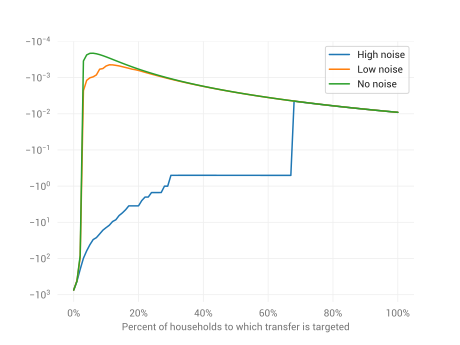
\includegraphics{by_noise_0_2_0}  % [width=15cm] 
	\captionof{figure}{CRRA by percent of households given transfer, 0.2\% of 
	GDP}
	\label{fig:by_noise_0_2_0}
\end{center}

\subsection{Allowing a portion of the budget to fund UBI} \label{ubi_portion}

In the baseline scenario (0.2 percent of GDP; low noise), social welfare is not 
improved when setting aside part of the budget for a UBI, nor is it improved 
with a noiseless signal. However, when noise is doubled, the previous optimum 
CRRA of $-0.0045$ can improve to $-0.0015$.
Without the option of reserving part for a UBI,
this high-noise scenario is optimized by targeting the bottom 68 
percent;
with the option, welfare is improved by directing 52 percent of the 
budget to a UBI, and targeting the remainder to the bottom 14 percent.

High-noise programs benefit substantially from diverting a share to a UBI, 
especially for smaller program budgets. For large program budgets, low-noise 
programs also benefit: CRRA rises 3.5 percent for a 1 percent of GDP program, 
and 8.3 percent for a 5 percent of GDP program.

\begin{center}
	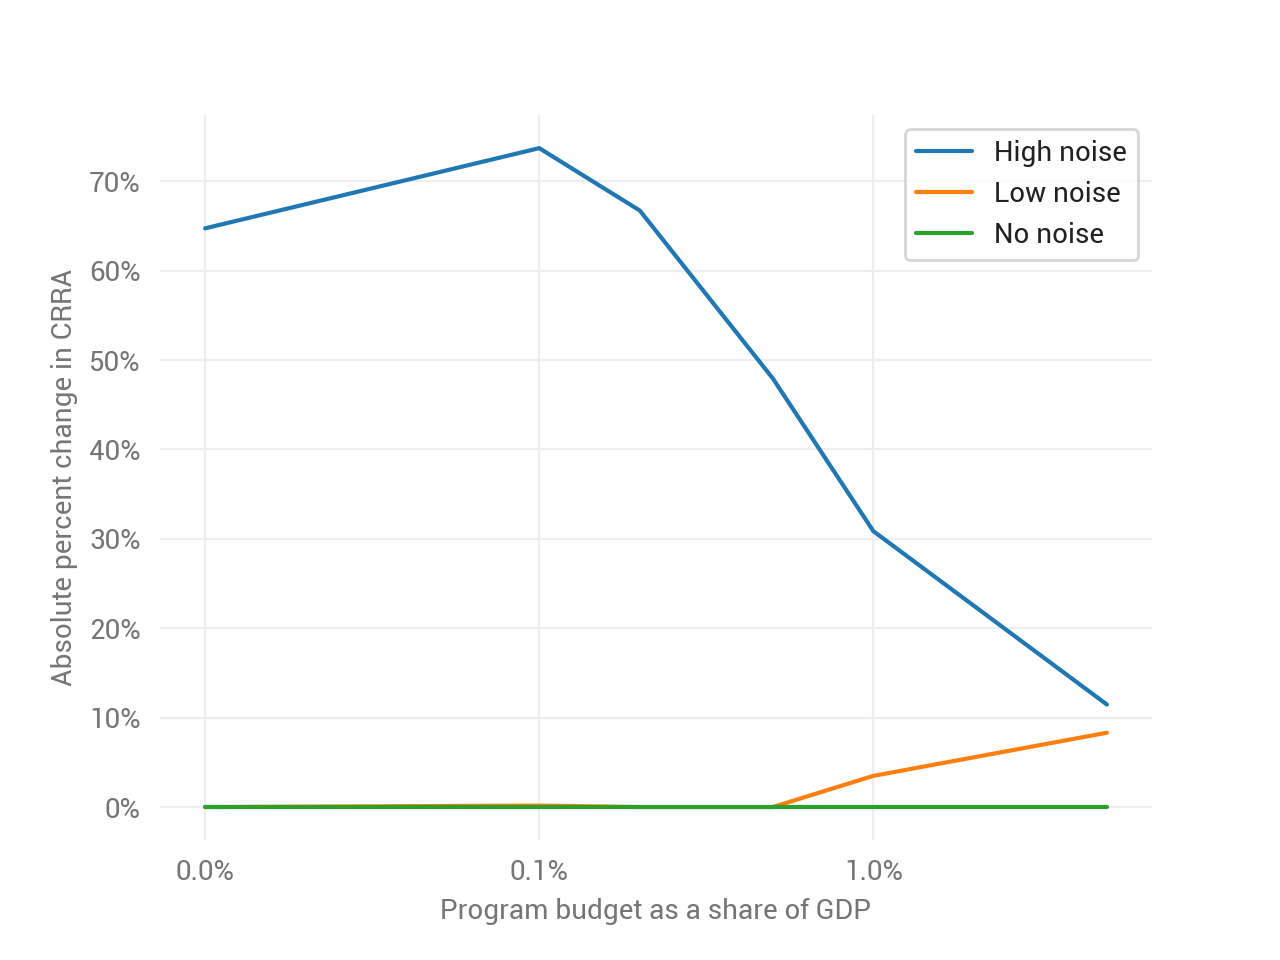
\includegraphics{improvement_from_partial_ubi}  % [width=15cm] 
	\captionof{figure}{CRRA improvement when allowing a portion of budget to 
	fund UBI}
	\label{fig:improvement_from_partial_ubi}
\end{center}

\section{Conclusion} \label{sec:conclusion}

I extend the approach of Hanna and Olken (2018), which optimizes social welfare 
by varying a program's targeting, by modeling different budget levels, noise 
levels, and the option to use part of the budget for a UBI.
I find that larger  programs generate greater social welfare by providing more 
generous transfers and by including more of the population.
Programs that only have access to a noisy signal should include more of the 
population,
though they will ultimately achieve less social welfare than sharper signals.
When the signal is noisy,
using part of the budget for a UBI can improve social welfare by
reducing exclusion errors;
the advantages of such a system are largest for small programs with
very noisy signals,
though they can also help for larger programs with less noisy signals.

This analysis does not consider horizontal equity, which Hanna and Olken define 
as the share of households with similar true consumption (e.g. within 5 
percentage points on the distribution) that get the same transfer amount. Hanna 
and Olken show that universal programs have greater horizontal equity. 
Reserving part of the program for a UBI will also improve horizontal equity 
(though a variable amount from the two components will require adjusting the 
definition). With a social welfare function that incorporates both utility 
(e.g. CRRA) and other measures like horizontal equity, the partial-UBI approach 
will be more attractive in more scenarios.



\clearpage

%\singlespacing
%\setlength\bibsep{0pt}

\bibliographystyle{apacite} % We choose the "plain" reference style.
\bibliography{refs} % Entries are in the "refs.bib" file.

\end{document}
